\documentclass[12pt]{article}
\usepackage{float}
\usepackage{graphicx}
\usepackage{fontspec}
\usepackage{titlesec}
\usepackage{setspace}
\usepackage[style=numeric,backend=biber,sorting=none]{biblatex}
\usepackage[a4paper, total={6in, 8in}, margin=0.5in]{geometry}
\addbibresource{ref.bib}

%%%%%%%% FORMAT
\singlespacing
\setmainfont{Arial}

\titleformat*{\section}{\normalsize\bfseries}
\titleformat*{\subsection}{\normalsize\bfseries}

\pagenumbering{gobble} % Suppress page number

% \titlespacing\section{0pt}{12pt plus 4pt minus 2pt}{0pt plus 2pt minus 2pt}
% \titlespacing\subsection{0pt}{12pt plus 4pt minus 2pt}{0pt plus 2pt minus 2pt}
% \titlespacing\subsubsection{0pt}{12pt plus 4pt minus 2pt}{0pt plus 2pt minus 2pt}


\begin{document}
  
%%%%%%%%% TITLE  
\title{\large Give a brief comparison on the innate and the adaptive defence systems \vspace{-2em}}
% \author{\large Yujia Shi\vspace{-1em}}
\date{\vspace{-2.5em}}
\maketitle

%%%%%%%%% BODY TEXT
\section{INTROUDCTION}

Our living environment is heavily filled with pathogenic and non-pathogenic microbs which includes a variety of toxic and allergenic substances to pose threat on normal homeostasis by replicating, spreading and threatening normal host functions. To recognize and destory those abnormal cells in our body, the immsune system is designed and evolved to defence against dangerous invader such as gerns, virus, cancer cells and organs and tissues transplanted, at the same time,they also avoid the immunse system casue enormous destruction on self-tissue that might elimate 
commensal microbes by detecting the mark of toxin it is distince from host cells or the structural features of the pathogen. \medskip

The immune system is a complex protective network consist of  white blood cells, antibodies, the complement system, the lymphatic system. Each of these elements is important to immune system, particularly for bone marrow and thymus.Both bone marrow and thymus are belong to primary lymphoid organs where to  generate and multiply two main of lymphocytes, which includes B and T cells.
Bone marrow is a spongy tissue which responsible to produce all body's blood cells, including B (mature in bond marrow) and T lymphocytes(mature in thymus). Different blood cells will work together within the immune system and  move to place needed to defence foreign substances in the body from the bone marrow;while for Thymus is a gland can be found above the heart and between the lungs. The Thymus eventually will replaced by connective tissue and fat, which only active in the stage of puberty and gradully slow down.The thymus is take charge of producing the hormone thym , and thereby assist in the generation of T cells.T cells are borned in the bone marrow and mature in thymus,after multiply in the thymus which will differntiate into helper, regulatory,  cytotoxic and memory T cells with different functions such as 
\begin{itemize}
    \item [1)] 
    CD4+ helper T cells : Be a helper cells to guide immunse system to attack invaders as rapidly and efficeiently as possbile, which also communicate with the B cells to produce antibodies.
    \item [2)]
    CD8+ killer T cells: Their daily routine work is directly destory countless cancer and virus-infected cells in the body.and equipped with the ability to distinguish the different between foreign molecules and body's own antigens
    \item [3)]
    Cytotoxic T cells:
    Cytotoxic cells is a type of white blood cell that are the main effector in adaptive immune system and are primarily activated by cytokines, so they can kill cells that are infected with virus or bacteria, cancer cells.
    \item [4)]
    Regulatory T cell:
    Regulatory T cell, also called Tregs, is capable of regulatoring and suppressing harmful cells, they are the key components help to prevent excessive immune response and autoimmune disease.
\end{itemize}
and equipped with the ability to distinguish the different between foreign molecules and body's own antigens.As T cells can identify self-structures and foreign antigens makes it become an critical elegant mechanism in immunse system.Apart from the tissue and organs component of bone marrow and thymus, other components comparised in immunse system also play critical role in making the system works smoothly,is capable of activating and moblilzing forces to prevent any  potential harmful susbstances such as toxic or allergenic substances enter through our mucosal surface.\medskip

Before taking action to response and control the pathogen microbes, toxin and exogenous threats, it is important for immune system to initial the mechanisms of self-nonself recognition, to differntiate self from non-self, in other words, is to distingush the antigens belong in our body from foreign antigenes such as toxins, chemicals, drugs which may envoking the immunse system called immunogens.The mechanisms of discrimination of self from nonself is not noly factilite thr the process to destory  or clear up a borad range harmful microbial cells, toxic and allergenic substances, but aslo to avoid these destructive mechanisms demage mammalian host's own tissue, resulting in broad class of autoimmune disorders.\medskip


Antigen, is a complex natural of protein substances that will binds particularly to a receptor molecule and mady by the body's infection-fightiing whitle blood cells(lymphocytes). Antigenes with molecules can be found on several places such as virus, bacteria and fungi, sometimes located on the surface of foreign substances, such as dust and organ tansplantation. A antigen may or may not stimulating an immune response, especially activating lymphocytes when it binds to a receptor molecule, even thogh a antigenes usualluy have diversity of three-dimensional patterns on distnct places of  their surfaces and each of pattern such as an antigenic determinant, or epitope has ability to stimulate different different lymphocyte receptor to  multiply and initate the an immune response, for example, the generation of antibodies or the activation of cytotoxic cells.Although the truth that some of antigenes can not evoke the immune system by temselves, but still helpful in the study of immunse response, as they can join with other larger and more complex  protein molecules to becomne immunogenic.General speaking, antigens can be divide into two main divisions: foregin(or heteroantigens) and antigenes.
Foregin antigens is coming from the outside of body,there are variety of substances can be classified into foreign antigens, example include the substance generated from virus, bacterial and protozoa, some of protein in foods, the serm and red blood cells components from other person. In contrast to foreign antigens,Autoantigens is reside within the body.\medskip

In generally, an indivdual without autoimmune disorders,his or her body is able to carry out the process of discriminting self from noself by inducing the immune system to generate the autoantibodies or destory the anitgen directly,which is called an immunogen.


 \begin{figure}[H]
    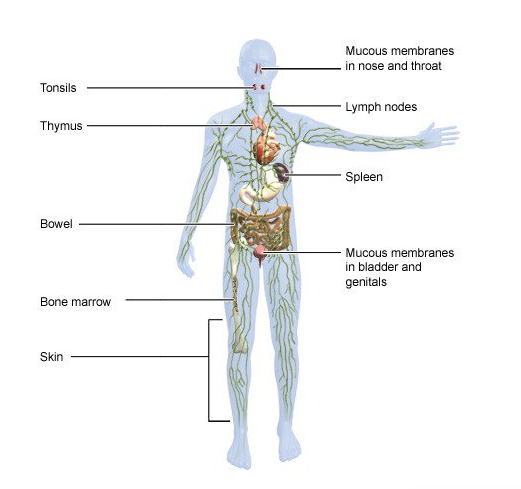
\includegraphics[width=0.7 \linewidth,height=0.62 \columnwidth]{/Users/yu-pinglin/Desktop/Essay/6001_Francis.png}
    \centering
    \caption{The 4 pillars for building a sustainable portfolio of
    core facilities.}
\end{figure}

\section{The innate and adaptive immune systems}
The immune response is made up of  two parts: the innate (non-specialized) immunity and the adaptive (specialized) immunity. The innate immunity response to an invader fast acting and non-sepcific, which is a immunity that a person is born with, while for the adaptive immunity which is not as immedicate as innate immunity, this type of immunity is usually slow to response a new invader at the very begining. Lymphocytes are the type of white blood cell (B and T cells) take charge of the adaptive immunity, when they first encounters foreign substances (antigens),they need time to learn, adapt and remember.The components of adaptive immunity will learn the best way to attack each invader and begin to estalish a memory for that invader.Thereafter, the respond will be improved beacuse the memroy is formed for the past invader, so B and T cells can identify previously encountered invader in a shorest of time, working together to desotry it even more efficeiently. \medskip

People usually describe the innate and adpative immune system as contrasting, separate arms of the host response;however,these two systems cooperate with each other and work on different tasks.


\subsection{Innate defence system}
The innate immune system offer a first-line barriers and non-specife response to keep potential pathogen, which include  viruses, bacteria, fungi, protozoans, and worm from entering you body. It acts very quickly to prevent the transmission and movement of germs and foreign substances throughout the body.For example, the innate system will destory a bacteria within a few hours, when it has entered to the skin via a sma;wound.The reson why the innate system referred as "nonspecific" immune system is that it responds in  the same way to specified virus and bacterial that it recognizes.The innate immune system provides nonspecific defense protection which is made up of a number of defense mechanisms,which include Physical barriers,Chemical barriers and Cellular defenses.
\begin{itemize}
    \item [1)] 
    Physical barriers : All outer and inner surfaces of our body are belong to the physical
    barriers, which is the first line of defence in fighting invasion by microbes and parasites. These include the skin and mucous membranes.Human skin include a outer layper of cell which is considered as mechanical barrier to infection.Furthermore, skin gland will secrete a variety of chemicals substances or enzyme,for example secrete oleic acid to kill bacterial or lysozyme to destory the outer wall of bacterial.There is a variety of mucous membranes surround our body organs, to protect the body from being infected and keep those tissue moisturized by secreting mucus.
    \item [2)]
    Chemical barriers: The primarily function of chemical barriers such as tears, mucous and stomach acid, is to harm and destory the invader which about to enter the internal tissues.
    \item [3)]
    Cellular barriers: The cellers in the innate immune system are nonspecific effectors cells such as scavanger cells and natural killer cells, they will neutralize  or destory those pathogens and substances that are likely dangerous to our body. 
\end{itemize}

\subsection{Adaptive defence system}
The adaptive defence system will becoming prominent defence after the first line of host denfence.
The second line of protection is called adaptive immunity, we also referred it as acquired immunity or sepcific immumity and is only found in vertebrates and will not always exits thorughout an individula’s entire lifespan.It is much slower to respond than the innate immunate response. as the adaptive immune response is the clonl expansion of T and B cells, which takes the body time to increase the number of T and  lymphocytes.However, it is more accute and robust than the innate immune system, the adaptive immune system is able to response faster when an indivdual met the some pathogen in the seond time.The increased speed is due to memory cells. 

\subsection{Innate vs adaptive immunity}
Give comparison between innate and adaptive defence system.The innate immunse response is immedicate with limited power to stop the spread of germs. the adaptive immune response is particularly sepcific, long-term(over 96 hours).In term of the cell types involved in both of immunity are different.In the innate immune response which includes macrophages, neutrophils, eosinophils;while for adaptive immune response  are based primarily on the antigen-specific receptors of T- and B-lymphocytes.

\section{CONCLUSION}
The immunse system consists of many components such as cellular  components,molecular components to protect us from a universe of pathogenic microbes.Understanding the function of different components will allows for improvement in vaccines,immunomodulatory therapeutics as well as avoidance of unexpected tissue injury.


\emergencystretch=1em
\printbibliography[title=Reference]

\end{document}




